\documentclass[journal]{IEEEtran}

\usepackage{amsmath,amssymb}
\usepackage{booktabs}
\usepackage{graphicx}
\usepackage{multirow}
\usepackage{siunitx}
\usepackage{xcolor}
\usepackage{cite}
\usepackage{url}
\usepackage{xspace}
\usepackage[hidelinks]{hyperref}
\usepackage{balance}
\usepackage{placeins}
\usepackage{tikz}
\usetikzlibrary{arrows.meta,positioning,fit,shapes.geometric}

\definecolor{stageblue}{HTML}{0072B2}
\definecolor{stageorange}{HTML}{D55E00}
\definecolor{stagegreen}{HTML}{009E73}
\definecolor{stagegray}{HTML}{555555}
\newcommand{\stagehci}[4]{%
  \draw[#4,line width=0.75pt] (#1,#3)--(#2,#3);
  \draw[#4,line width=0.75pt] (#1,#3-0.09)--(#1,#3+0.09);
  \draw[#4,line width=0.75pt] (#2,#3-0.09)--(#2,#3+0.09);
}
\newcommand{\stagevci}[4]{%
  \draw[#4,line width=0.75pt] (#3,#1)--(#3,#2);
  \draw[#4,line width=0.75pt] (#3-0.09,#1)--(#3+0.09,#1);
  \draw[#4,line width=0.75pt] (#3-0.09,#2)--(#3+0.09,#2);
}
\newcommand{\StagePairedFallback}{%
\resizebox{\textwidth}{!}{%
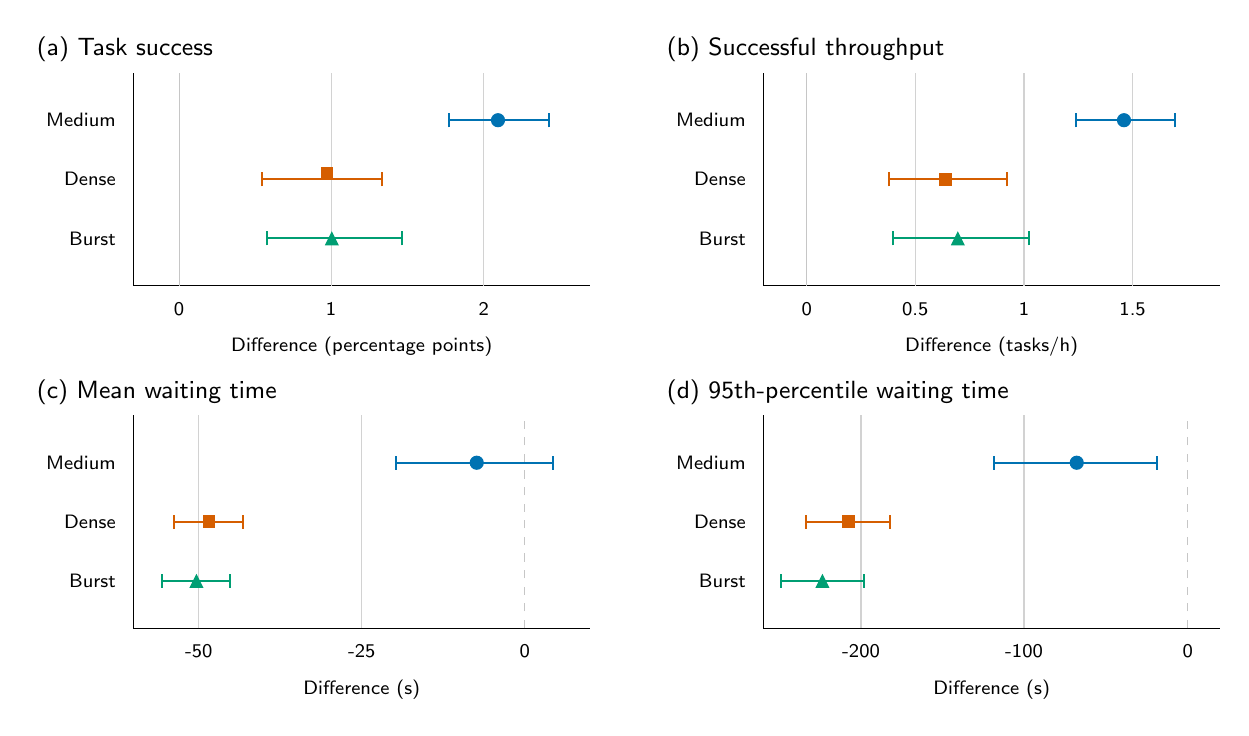
\begin{tikzpicture}[font=\sffamily\scriptsize]
  \begin{scope}[shift={(0,4.35)}]
    \node[anchor=west,font=\sffamily\small] at (0,3.65) {(a) Task success};
    \draw (1.35,0.65)--(7.15,0.65); \draw (1.35,0.65)--(1.35,3.35);
    \draw[gray!45] (1.93,0.65)--(1.93,3.35);
    \draw[gray!35] (3.86,0.65)--(3.86,3.35);
    \draw[gray!35] (5.80,0.65)--(5.80,3.35);
    \node[anchor=east] at (1.25,2.75) {Medium};
    \node[anchor=east] at (1.25,2.00) {Dense};
    \node[anchor=east] at (1.25,1.25) {Burst};
    \node[anchor=north] at (1.93,0.56) {0};
    \node[anchor=north] at (3.86,0.56) {1};
    \node[anchor=north] at (5.80,0.56) {2};
    \node[anchor=north] at (4.25,0.12) {Difference (percentage points)};
    \stagehci{5.36}{6.63}{2.75}{stageblue}
    \stagehci{2.98}{4.51}{2.00}{stageorange}
    \stagehci{3.05}{4.76}{1.25}{stagegreen}
    \fill[stageblue] (5.98,2.75) circle (0.09);
    \fill[stageorange] (3.73,2.00) rectangle +(0.16,0.16);
    \fill[stagegreen] (3.87,1.34)--(3.78,1.16)--(3.96,1.16)--cycle;
  \end{scope}
  \begin{scope}[shift={(8.0,4.35)}]
    \node[anchor=west,font=\sffamily\small] at (0,3.65) {(b) Successful throughput};
    \draw (1.35,0.65)--(7.15,0.65); \draw (1.35,0.65)--(1.35,3.35);
    \draw[gray!45] (1.90,0.65)--(1.90,3.35);
    \draw[gray!35] (3.28,0.65)--(3.28,3.35);
    \draw[gray!35] (4.66,0.65)--(4.66,3.35);
    \draw[gray!35] (6.04,0.65)--(6.04,3.35);
    \node[anchor=east] at (1.25,2.75) {Medium};
    \node[anchor=east] at (1.25,2.00) {Dense};
    \node[anchor=east] at (1.25,1.25) {Burst};
    \node[anchor=north] at (1.90,0.56) {0};
    \node[anchor=north] at (3.28,0.56) {0.5};
    \node[anchor=north] at (4.66,0.56) {1};
    \node[anchor=north] at (6.04,0.56) {1.5};
    \node[anchor=north] at (4.25,0.12) {Difference (tasks/h)};
    \stagehci{5.32}{6.58}{2.75}{stageblue}
    \stagehci{2.95}{4.45}{2.00}{stageorange}
    \stagehci{3.00}{4.72}{1.25}{stagegreen}
    \fill[stageblue] (5.93,2.75) circle (0.09);
    \fill[stageorange] (3.58,1.92) rectangle +(0.16,0.16);
    \fill[stagegreen] (3.82,1.34)--(3.73,1.16)--(3.91,1.16)--cycle;
  \end{scope}
  \begin{scope}
    \node[anchor=west,font=\sffamily\small] at (0,3.65) {(c) Mean waiting time};
    \draw (1.35,0.65)--(7.15,0.65); \draw (1.35,0.65)--(1.35,3.35);
    \draw[gray!35] (2.18,0.65)--(2.18,3.35);
    \draw[gray!35] (4.25,0.65)--(4.25,3.35);
    \draw[gray!45,dashed] (6.32,0.65)--(6.32,3.35);
    \node[anchor=east] at (1.25,2.75) {Medium};
    \node[anchor=east] at (1.25,2.00) {Dense};
    \node[anchor=east] at (1.25,1.25) {Burst};
    \node[anchor=north] at (2.18,0.56) {-50};
    \node[anchor=north] at (4.25,0.56) {-25};
    \node[anchor=north] at (6.32,0.56) {0};
    \node[anchor=north] at (4.25,0.12) {Difference (s)};
    \stagehci{4.68}{6.68}{2.75}{stageblue}
    \stagehci{1.87}{2.74}{2.00}{stageorange}
    \stagehci{1.71}{2.58}{1.25}{stagegreen}
    \fill[stageblue] (5.71,2.75) circle (0.09);
    \fill[stageorange] (2.23,1.92) rectangle +(0.16,0.16);
    \fill[stagegreen] (2.15,1.34)--(2.06,1.16)--(2.24,1.16)--cycle;
  \end{scope}
  \begin{scope}[shift={(8.0,0)}]
    \node[anchor=west,font=\sffamily\small] at (0,3.65) {(d) 95th-percentile waiting time};
    \draw (1.35,0.65)--(7.15,0.65); \draw (1.35,0.65)--(1.35,3.35);
    \draw[gray!35] (2.59,0.65)--(2.59,3.35);
    \draw[gray!35] (4.66,0.65)--(4.66,3.35);
    \draw[gray!45,dashed] (6.74,0.65)--(6.74,3.35);
    \node[anchor=east] at (1.25,2.75) {Medium};
    \node[anchor=east] at (1.25,2.00) {Dense};
    \node[anchor=east] at (1.25,1.25) {Burst};
    \node[anchor=north] at (2.59,0.56) {-200};
    \node[anchor=north] at (4.66,0.56) {-100};
    \node[anchor=north] at (6.74,0.56) {0};
    \node[anchor=north] at (4.25,0.12) {Difference (s)};
    \stagehci{4.28}{6.35}{2.75}{stageblue}
    \stagehci{1.89}{2.96}{2.00}{stageorange}
    \stagehci{1.57}{2.63}{1.25}{stagegreen}
    \fill[stageblue] (5.33,2.75) circle (0.09);
    \fill[stageorange] (2.35,1.92) rectangle +(0.16,0.16);
    \fill[stagegreen] (2.10,1.34)--(2.01,1.16)--(2.19,1.16)--cycle;
  \end{scope}
\end{tikzpicture}}}
\newcommand{\StageAdaptFallback}{%
\resizebox{\textwidth}{!}{%
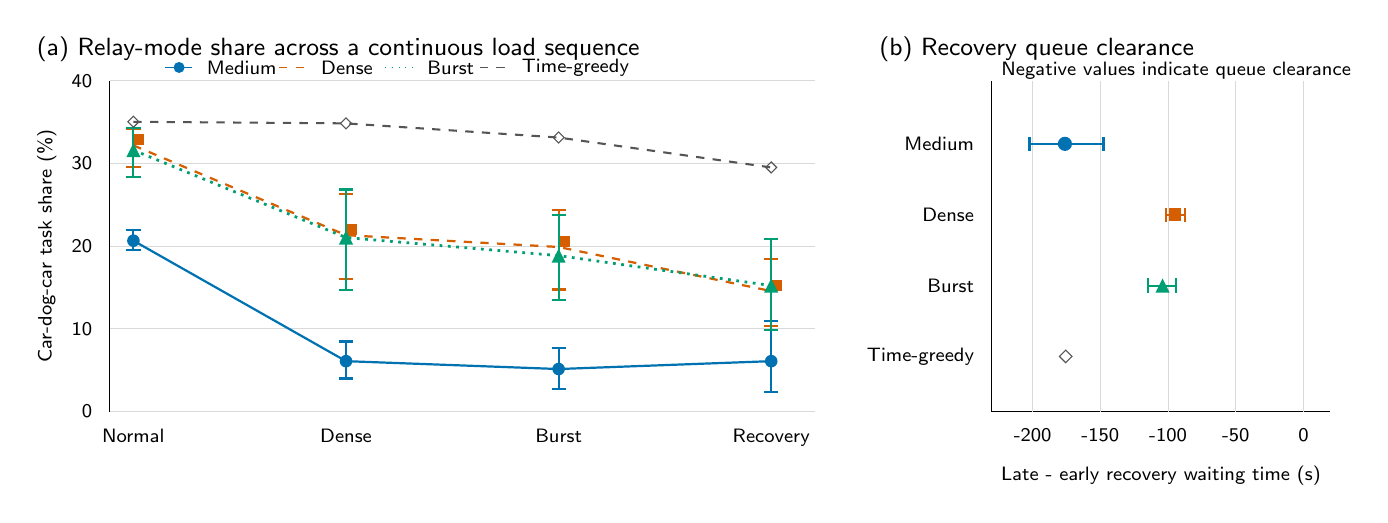
\begin{tikzpicture}[font=\sffamily\scriptsize]
  \begin{scope}
    \node[anchor=west,font=\sffamily\small] at (0,5.35) {(a) Relay-mode share across a continuous load sequence};
    \draw (1.05,0.75)--(10.0,0.75); \draw (1.05,0.75)--(1.05,4.95);
    \foreach \yy/\lab in {0.75/0,1.80/10,2.85/20,3.90/30,4.95/40}{
      \draw[gray!30] (1.05,\yy)--(10.0,\yy);
      \node[anchor=east] at (0.95,\yy) {\lab};
    }
    \node[rotate=90] at (0.25,2.85) {Car-dog-car task share (\%)};
    \foreach \xx/\lab in {1.35/Normal,4.05/Dense,6.75/Burst,9.45/Recovery}{
      \node[anchor=north] at (\xx,0.65) {\lab};
    }
    \stagevci{2.80}{3.06}{1.35}{stageblue}
    \stagevci{1.17}{1.64}{4.05}{stageblue}
    \stagevci{1.04}{1.56}{6.75}{stageblue}
    \stagevci{1.00}{1.90}{9.45}{stageblue}
    \draw[stageblue,line width=0.8pt] (1.35,2.92)--(4.05,1.39)--(6.75,1.29)--(9.45,1.39);
    \foreach \p in {(1.35,2.92),(4.05,1.39),(6.75,1.29),(9.45,1.39)}{\fill[stageblue] \p circle (0.08);}
    \stagevci{3.86}{4.34}{1.35}{stageorange}
    \stagevci{2.43}{3.51}{4.05}{stageorange}
    \stagevci{2.30}{3.31}{6.75}{stageorange}
    \stagevci{1.84}{2.69}{9.45}{stageorange}
    \draw[stageorange,dashed,line width=0.8pt] (1.35,4.13)--(4.05,2.99)--(6.75,2.84)--(9.45,2.28);
    \foreach \p in {(1.35,4.13),(4.05,2.99),(6.75,2.84),(9.45,2.28)}{\fill[stageorange] \p rectangle +(0.14,0.14);}
    \stagevci{3.73}{4.35}{1.35}{stagegreen}
    \stagevci{2.29}{3.57}{4.05}{stagegreen}
    \stagevci{2.17}{3.25}{6.75}{stagegreen}
    \stagevci{1.78}{2.94}{9.45}{stagegreen}
    \draw[stagegreen,dotted,line width=1.0pt] (1.35,4.07)--(4.05,2.96)--(6.75,2.73)--(9.45,2.35);
    \foreach \x/\y in {1.35/4.07,4.05/2.96,6.75/2.73,9.45/2.35}{
      \fill[stagegreen] (\x,\y+0.09)--(\x-0.09,\y-0.09)--(\x+0.09,\y-0.09)--cycle;
    }
    \draw[stagegray,dashed,line width=0.75pt] (1.35,4.43)--(4.05,4.41)--(6.75,4.23)--(9.45,3.85);
    \foreach \p in {(1.35,4.43),(4.05,4.41),(6.75,4.23),(9.45,3.85)}{\draw[stagegray] \p ++(-0.07,0)--++(0.07,0.07)--++(0.07,-0.07)--++(-0.07,-0.07)--cycle;}
    \draw[stageblue] (1.75,5.12)--(2.10,5.12); \fill[stageblue] (1.93,5.12) circle (0.07); \node[anchor=west] at (2.16,5.12) {Medium};
    \draw[stageorange,dashed] (3.20,5.12)--(3.55,5.12); \node[anchor=west] at (3.61,5.12) {Dense};
    \draw[stagegreen,dotted] (4.55,5.12)--(4.90,5.12); \node[anchor=west] at (4.96,5.12) {Burst};
    \draw[stagegray,dashed] (5.75,5.12)--(6.10,5.12); \node[anchor=west] at (6.16,5.12) {Time-greedy};
  \end{scope}
  \begin{scope}[shift={(10.7,0)}]
    \node[anchor=west,font=\sffamily\small] at (0,5.35) {(b) Recovery queue clearance};
    \node[anchor=west] at (1.55,5.08) {Negative values indicate queue clearance};
    \draw (1.55,0.75)--(5.85,0.75); \draw (1.55,0.75)--(1.55,4.95);
    \foreach \xx/\lab in {2.07/-200,2.93/-150,3.79/-100,4.65/-50,5.51/0}{
      \draw[gray!30] (\xx,0.75)--(\xx,4.95);
      \node[anchor=north] at (\xx,0.65) {\lab};
    }
    \node[anchor=east] at (1.45,4.15) {Medium};
    \node[anchor=east] at (1.45,3.25) {Dense};
    \node[anchor=east] at (1.45,2.35) {Burst};
    \node[anchor=east] at (1.45,1.45) {Time-greedy};
    \node[anchor=north] at (3.70,0.18) {Late - early recovery waiting time (s)};
    \stagehci{2.03}{2.97}{4.15}{stageblue}
    \stagehci{3.76}{4.01}{3.25}{stageorange}
    \stagehci{3.54}{3.89}{2.35}{stagegreen}
    \fill[stageblue] (2.48,4.15) circle (0.09);
    \fill[stageorange] (3.80,3.17) rectangle +(0.16,0.16);
    \fill[stagegreen] (3.72,2.44)--(3.63,2.26)--(3.81,2.26)--cycle;
    \draw[stagegray] (2.41,1.45)--(2.49,1.53)--(2.57,1.45)--(2.49,1.37)--cycle;
  \end{scope}
\end{tikzpicture}}}

\hypersetup{
  pdftitle={Event-Driven Masked SMDP-PPO for Persistent Heterogeneous Multi-Robot Transport in a Multi-Floor Warehouse},
  pdfauthor={},
  pdfsubject={Anonymous submission to IEEE Transactions on Robotics},
  pdfkeywords={multi-robot systems, task allocation, reinforcement learning, warehouse automation}
}

% Let wide evidence appear near its first citation without turning Results into
% a sequence of forced float pages.  A single barrier remains at the end of
% Results; no intermediate clear-page behavior is imposed.
\setcounter{topnumber}{2}
\setcounter{dbltopnumber}{2}
\renewcommand{\topfraction}{0.85}
\renewcommand{\dbltopfraction}{0.88}
\renewcommand{\textfraction}{0.10}
\renewcommand{\floatpagefraction}{0.72}
\renewcommand{\dblfloatpagefraction}{0.75}
\setlength{\textfloatsep}{10pt plus 2pt minus 2pt}
\setlength{\dbltextfloatsep}{10pt plus 2pt minus 2pt}
\makeatletter
\setlength{\@dblfptop}{0pt}
\setlength{\@dblfpsep}{10pt plus 2pt minus 2pt}
\setlength{\@dblfpbot}{0pt plus 1fil}
\makeatother

% xspace prevents mode names from swallowing a following word while retaining
% correct spacing before punctuation and explicit braces.
\DeclareRobustCommand{\method}{E-SMDP-PPO\xspace}
\DeclareRobustCommand{\modecar}{\mbox{\textsc{Single-Car}}\xspace}
\DeclareRobustCommand{\modedog}{\mbox{\textsc{Single-Dog}}\xspace}
\DeclareRobustCommand{\modechain}{\mbox{\textsc{Car--Dog--Car}}\xspace}

\title{Event-Driven Masked SMDP-PPO for Persistent Heterogeneous Multi-Robot Transport in a Multi-Floor Warehouse}
\author{}

\begin{document}

% The anonymous journal draft has no author block; remove the vertical space
% that IEEEtran would otherwise reserve beneath the title.
\IEEEaftertitletext{\vspace{-2\baselineskip}}
\maketitle

\begin{abstract}
Multi-floor warehouses couple task allocation with transport-mode selection: wheeled robots move efficiently on level ground, legged robots traverse stairs, and cross-floor deliveries may use one legged robot or a wheeled--legged--wheeled relay. We formulate this problem as an event-driven semi-Markov decision process with asynchronous arrivals, variable-duration actions, persistent robot locations, and concurrent resource use. At each decision epoch, a centralized policy selects a task, mode, participating robots, and stairway. A feasibility layer enumerates joint candidates and masks conflicts before sampling. A shared actor combines global context with per-candidate geometric, temporal, resource, and handover-risk features. Proximal policy optimization uses duration-aware discounting and generalized advantage estimation. Locked tests retain 30 fixed-profile and ten mixed-curriculum policies, each evaluated on 100 shared streams. The mixed-curriculum cohort maintains 96.51\% success in randomized persistent mixed load, statistically comparable to a time-greedy rule, while reducing mean waiting by 30.14~s. Under a second frozen evaluation covering a no-fault control and three logical fault conditions, PPO and time-greedy success and throughput remain comparable, while PPO reduces mean waiting by 29.76--34.43~s and P95 waiting by 122.65--138.51~s. Across 54 fixed-shape CPU benchmarks, the worst scheduling-decision p99 is 4.815~ms. The policy operates only at the scheduling layer; navigation and robot control remain separate.
\end{abstract}

\begin{IEEEkeywords}
Multi-robot systems, task allocation, reinforcement learning, warehouse automation.
\end{IEEEkeywords}

\section{Introduction}
\label{sec:introduction}

Warehouses increasingly combine robots with complementary mobility and payload characteristics. Wheeled platforms can transport goods quickly and efficiently on planar aisles, whereas legged platforms can negotiate stairs and other discontinuities that remain inaccessible to conventional mobile bases. This complementarity is particularly useful in existing multi-floor facilities, where installing lifts or conveyors may be costly or infeasible. It also creates a scheduling problem that is more tightly coupled than assigning each task to its nearest available robot. A cross-floor delivery may be completed by one legged robot, or decomposed into a source-floor wheeled segment, a legged stair segment, and a destination-floor wheeled segment. The second option can reduce travel time but occupies more robots and introduces two handovers, synchronization requirements, and additional failure exposure.

The resulting decision problem combines several aspects of multi-robot task allocation (MRTA). Tasks arrive online rather than as a fixed batch; robot positions and workloads persist across assignments; several tasks may execute concurrently; and the duration of a joint assignment depends on the selected mode and on the slowest synchronized branch. Decisions therefore affect not only the current delivery but also the future spatial distribution of the fleet and the availability of stairs, handover regions, and standby locations. A policy optimized for an isolated task can create queues or resource conflicts later in the episode.

Classical MRTA methods provide principled formulations for heterogeneous capabilities, temporal constraints, coalitions, and plan repair. Recent learning-based work has improved responsiveness in dynamic warehouses and has addressed heterogeneous coalitions or asynchronous macro-actions. However, the combination considered here remains distinctive: the high-level controller must choose among direct wheeled transport, direct legged transport, and an explicit wheeled--legged--wheeled relay while respecting shared stair and handover resources under continuous asynchronous arrivals. The action is combinatorial, but the set of feasible assignments changes at every event.

We address this setting with an event-driven semi-Markov decision process (SMDP). The transition duration is part of each experience tuple, so discounting reflects elapsed simulated time rather than an arbitrary count of scheduler calls. Feasible task--mode--robot--stair assignments are generated from the current system state. Invalid assignments are removed by a deterministic mask before the policy samples an action. Instead of attaching parameters to transient action indices, a shared actor scores each candidate from its own features and an explicit interaction with a global state embedding. This representation preserves the structure of the joint decision while allowing the legal candidate set to vary across events.

This paper makes three methodological contributions and one empirical contribution:
\begin{itemize}
  \item We formulate persistent, asynchronous transport in a multi-floor heterogeneous warehouse as a continuous-time SMDP in which a single high-level action jointly selects the task, transport mode, robots, and stairway.
  \item We develop a feasibility-preserving candidate representation for three transport modes---\modecar, \modedog, and \modechain---with deterministic resource and ownership constraints applied before policy sampling.
  \item We introduce a context-interaction actor that shares parameters across as many as 1536 dynamic candidates and is trained with duration-aware PPO and generalized advantage estimation.
  \item We provide a frozen, multi-seed evaluation across nonstationary load, mixed-regime generalization, fixed-shape scheduling latency, and logical fault injection, while separating this scheduling evidence from future navigation- and hardware-level validation.
\end{itemize}

The present system is a high-level scheduling contribution. The policy does not output joint torques, footholds, or velocity commands. Navigation is delegated to an external planner, and cargo transfer is represented by a transactional ownership model. These boundaries are stated explicitly so that logical scheduling evidence is not mistaken for contact-dynamics or hardware validation.

\section{Related Work}
\label{sec:related_work}

\subsection{Heterogeneous Task Allocation and Coalition Scheduling}

MRTA taxonomies characterize allocation problems according to robot multiplicity, task multiplicity, assignment dynamics, and inter-task constraints~\cite{gerkey2004taxonomy,korsah2013taxonomy}. Market-based coordination provides a complementary distributed perspective: auctions expose local execution costs~\cite{dias2006market}, while task-tree abstractions allow complex tasks to be decomposed and traded at different granularities~\cite{zlot2006market}. Behavior-based systems such as ALLIANCE instead emphasize adaptive task selection and graceful recovery from team-member failures~\cite{parker1994alliance}.

Heterogeneous teams extend the problem because feasibility and utility depend on complementary capabilities rather than distance alone. Notomista \emph{et al.}~\cite{notomista2022resilient} represent capabilities in an energy-aware allocation framework, while Fu \emph{et al.}~\cite{fu2023robust} jointly optimize decomposition, assignment, and scheduling under capability uncertainty. Aswale and Pinciroli~\cite{aswale2023coalition} study synchronization and heterogeneous travel times in multi-skilled coalitions. Dai \emph{et al.}~\cite{dai2025heterogeneous} learn dynamic coalitions for individual and collaborative tasks.

Capability-centered coalition systems provide an earlier foundation for this viewpoint. ASyMTRe synthesizes heterogeneous coalitions by composing sensory, computational, communication, and motor schemas rather than treating a robot as one indivisible capability label~\cite{parker2006asymtre}. IQ-ASyMTRe further reasons about interaction constraints so that a proposed tightly coupled coalition is executable in the current robot--environment configuration~\cite{zhang2013iqasymtre}. Our candidate generator follows the same feasibility-first principle at a coarser scheduling level: only complete transport chains whose morphology, floor, stair, handover, and ownership constraints are currently satisfiable are exposed to the policy.

Several works also integrate allocation with temporal or motion-level constraints. SCoBA interleaves planning and execution for dynamically arriving tasks with uncertain outcomes and temporal requirements~\cite{choudhury2022dynamic}. D-ITAGS combines allocation, scheduling, and motion planning, then repairs solutions locally after failures or delays~\cite{neville2023ditags}. Calvo and Capit\'{a}n~\cite{calvo2025longendurance} formulate long-endurance heterogeneous MRTA with charging, task fragmentation, coalitions, relays, and online replanning. The service-agent--transport-agent problem couples routes, docking, deployment, and robust timing in a mixed-integer program~\cite{bays2017satp}; more recently, mobile manipulators and transport agents have been dynamically paired for object transfer~\cite{yi2025tidying}. These approaches motivate explicit temporal feasibility and relay modeling. Our focus differs in learning an event policy that selects direct versus two-handover relay transport for a continuing warehouse stream.

The closest morphology-level example is the reactive allocation architecture of Zhou \emph{et al.}~\cite{zhou2022reactive}, which teams quadrupedal and wheeled delivery robots and handles execution failures. Oliveira \emph{et al.}~\cite{oliveira2022warehouse} consider heterogeneous robot speeds and loads in smart warehouses with multiple delivery stations. We retain this concern for heterogeneous travel time, but additionally model stair resources and two transactional handovers as part of a single candidate action.

\subsection{Learning for Dynamic Warehouse Scheduling}

Large-scale warehouse systems first highlighted the need to coordinate hundreds of continuously operating robots~\cite{wurman2007warehouse}. Lifelong multi-agent pickup-and-delivery formalizes a stream of online assignments coupled to collision-free paths~\cite{ma2017lifelong}; PRIMAL$_2$ learns decentralized lifelong pathfinding policies for dense, structured warehouses~\cite{damani2021primal2}. These works address assignment--routing interaction below or beside our scheduler, whereas our logical SMDP currently estimates travel time and evaluates navigation separately.

Learning-based MRTA can amortize repeated combinatorial decisions when task and fleet states evolve online. RTAW uses attention and PPO for warehouse allocation and triggers decisions as robots become available~\cite{agrawal2023rtaw}. HeuRAL-MATE combines a learned task selector with heuristic robot selection~\cite{pal2024heuristic}, while MRTAgent coordinates learned task and robot choices for real-time allocation~\cite{pal2025together}. Krnjaic \emph{et al.}~\cite{krnjaic2024scalable} use hierarchical MARL for warehouse logistics involving robotic and human co-workers. These methods are important baselines, but do not explicitly choose between a direct legged route and a three-robot, two-handover cross-floor chain.

Learning in heterogeneous teams must also account for partial observability, credit assignment, and temporal asynchrony. Zhang \emph{et al.}~\cite{zhang2024asynchronous} address heterogeneous macro-actions with different durations and asynchronous termination, while Jose and Zhang~\cite{jose2024learning} study dynamic subteaming and voluntary waiting. Earlier decentralized recurrent learning addresses partial observability and multi-task transfer~\cite{omidshafiei2017multitask}. Under centralized training and decentralized execution, MADDPG conditions critics on other agents' actions~\cite{lowe2017maddpg}, COMA uses a counterfactual baseline for credit assignment~\cite{foerster2018coma}, and QMIX factorizes a joint value monotonically into per-agent utilities~\cite{rashid2018qmix}.

PPO-based multi-agent methods provide an important neighboring family. MAPPO is a strong empirical baseline~\cite{yu2022mappo}; HATRPO and HAPPO use sequential updates without requiring shared policies~\cite{kuba2022happo}; and Bezerra \emph{et al.}~\cite{bezerra2025dynamic} extend MAPPO with intention sharing and spatial action maps for dynamic coalition formation. More directly addressing long-duration asynchrony, Xiao \emph{et al.}~\cite{xiao2025asynchronous} develop value- and policy-based MARL for asynchronously terminating macro-actions, while CATMiP combines class-based macro-actions with transformer coordination for heterogeneous teams~\cite{farjadnasab2025catmip}. These methods learn decentralized per-agent decisions. In contrast, our high-level implementation contains one centralized actor and critic; one decision selects a complete feasible task--mode--robot--stair tuple. We therefore describe it as centralized masked SMDP-PPO, not MAPPO or HAPPO.

\subsection{Navigation Execution Layer}

At the execution layer, SCAN-Planner combines yaw-aware whole-body collision checking, projected-A* guidance, B-spline trajectory optimization, and a robot-centric sliding occupancy map for route-guided quadruped navigation~\cite{zheng2026scan}. Its rebound-style optimization and sliding-map design are related to EGO-Planner~\cite{zhou2021egoplanner} and ROG-Map~\cite{ren2024rogmap}, respectively. Terrain-aware legged planners such as ArtPlanner~\cite{wellhausen2023artplanner} and multi-goal frameworks such as SMUG~\cite{chen2023smug} address complementary navigation-level problems. Our policy operates above this layer: it selects tasks, transport modes, robots, and stair resources, while continuous route generation remains outside the learned action space.

\subsection{Event-Driven Decision Making}

Discrete-time approximations can distort a system in which actions last from seconds to minutes. Generalized semi-Markov models represent asynchronous concurrent activities through events and variable holding times~\cite{messias2013gsmdp}. We adopt the same continuous-time motivation but optimize a neural policy with PPO~\cite{schulman2017ppo}. Generalized advantage estimation (GAE) reduces variance in policy-gradient updates~\cite{schulman2016gae}; here, both the temporal-difference residual and the recursive advantage use the transition-specific SMDP discount. This is important because a short wait and a multi-stage relay should not consume the same amount of discounted time merely because each produces one scheduler transition.

\begin{table*}[!t]
\centering
\caption{Positioning relative to representative related work. A filled circle denotes an explicit focus; an open circle denotes partial coverage. ``Relay choice'' means that allocation chooses between direct service and an inter-robot relay, rather than assuming a fixed collaboration pattern.}
\label{tab:related_comparison}
\footnotesize
\setlength{\tabcolsep}{3.5pt}
\begin{tabular}{lcccccc}
\toprule
Work & Hetero. & Online & Async. duration & Learning & Relay choice & Warehouse \\
\midrule
SCoBA~\cite{choudhury2022dynamic} & \textcolor{black}{$\bullet$} & \textcolor{black}{$\bullet$} & \textcolor{black}{$\circ$} & -- & -- & -- \\
D-ITAGS~\cite{neville2023ditags} & \textcolor{black}{$\bullet$} & \textcolor{black}{$\circ$} & \textcolor{black}{$\circ$} & -- & -- & -- \\
Calvo and Capit\'{a}n~\cite{calvo2025longendurance} & \textcolor{black}{$\bullet$} & \textcolor{black}{$\bullet$} & \textcolor{black}{$\circ$} & -- & \textcolor{black}{$\bullet$} & -- \\
RTAW~\cite{agrawal2023rtaw} & -- & \textcolor{black}{$\bullet$} & \textcolor{black}{$\circ$} & \textcolor{black}{$\bullet$} & -- & \textcolor{black}{$\bullet$} \\
Dai \emph{et al.}~\cite{dai2025heterogeneous} & \textcolor{black}{$\bullet$} & \textcolor{black}{$\circ$} & \textcolor{black}{$\circ$} & \textcolor{black}{$\bullet$} & -- & -- \\
Async MARL~\cite{zhang2024asynchronous} & \textcolor{black}{$\bullet$} & \textcolor{black}{$\circ$} & \textcolor{black}{$\bullet$} & \textcolor{black}{$\bullet$} & -- & -- \\
This work & \textcolor{black}{$\bullet$} & \textcolor{black}{$\bullet$} & \textcolor{black}{$\bullet$} & \textcolor{black}{$\bullet$} & \textcolor{black}{$\bullet$} & \textcolor{black}{$\bullet$} \\
\bottomrule
\end{tabular}
\end{table*}

\section{System and Problem Formulation}
\label{sec:problem}

\subsection{Warehouse and Robot Team}

We consider a two-floor warehouse served by a heterogeneous team $\mathcal{R}=\mathcal{R}^{c}\cup\mathcal{R}^{d}$. The first floor spans \SI{48}{m}$\times$\SI{40}{m}; the second spans \SI{30}{m}$\times$\SI{24}{m} at a height of \SI{4}{m} and contains an \SI{8}{m}$\times$\SI{6}{m} central void. Four external \SI{1.4}{m}-wide stairways connect the floors. The current configuration contains six wheeled Carter robots and four Unitree Go2 quadrupeds. Four Carter robots start on the first floor and two on the second floor. Carter and Go2 nominal translational speeds are \SI{2.0}{m/s} and \SI{0.8}{m/s}, respectively. Carter robots are restricted to level-ground motion; Go2 robots may move on either floor and traverse stairs.

\begin{figure*}[!t]
\centering
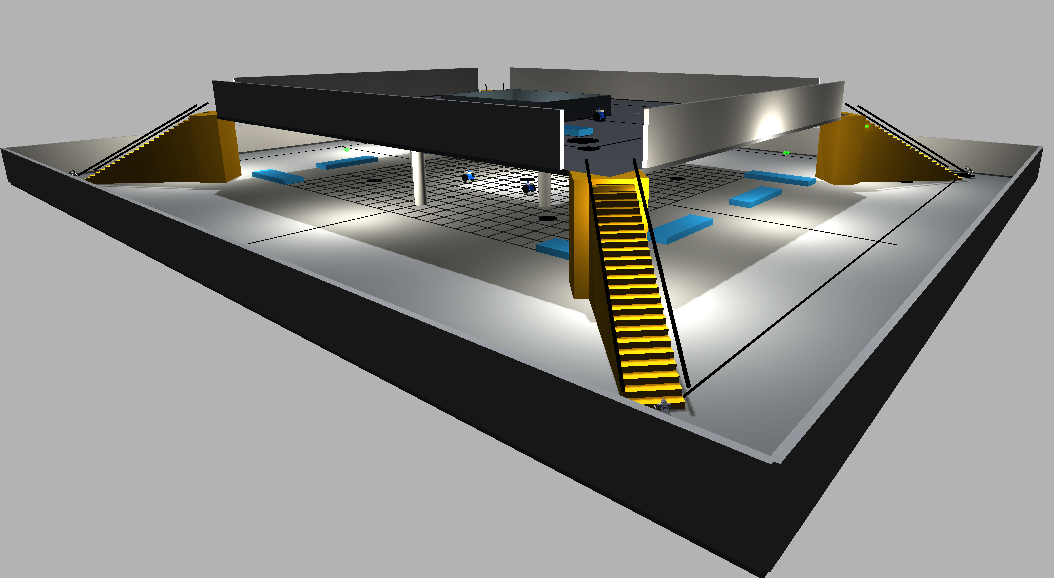
\includegraphics[width=0.82\textwidth]{warehouse_simulation_overview.png}
\caption{Project-generated overview of the two-floor warehouse simulation model. The scene contains the lower and upper work areas, a central opening, and four exterior stair connections used by the scheduling model. This image documents the modeled environment; the quantitative studies are produced by the logical continuous-time scheduler described in Section~\ref{sec:protocol}.}
\label{fig:warehouse_overview}
\end{figure*}

Navigation-level integration is evaluated separately from policy training using a project-adapted community ROS~2 port of SCAN-Planner~\cite{zheng2026scan}. In the archived route gates, both morphologies consume a static warehouse point cloud and preset waypoint sequences; morphology-specific envelopes and speed limits parameterize the planner, and the resulting B-spline trajectories are replayed by an open-loop controller. These trials test planner interfaces and kinematic route reachability, not sensor-closed-loop or contact-dynamics navigation. SCAN-Planner's published validation concerns a Unitree Go2; the Carter interface is an engineering adaptation in this project, not evidence that the original planner natively supports wheeled platforms.

A task $i$ is released at time $a_i$ and is described by
\begin{equation}
  q_i=(p_i^{\mathrm{s}},p_i^{\mathrm{g}},\ell_i^{\mathrm{s}},
  \ell_i^{\mathrm{g}},\rho_i,d_i),
\end{equation}
where $p_i^{\mathrm{s}}$ and $p_i^{\mathrm{g}}$ are source and goal coordinates, $\ell_i^{\mathrm{s}}$ and $\ell_i^{\mathrm{g}}$ are floors, $\rho_i$ is priority, and $d_i$ is a deadline. Tasks are not pre-labeled with a transport mode. The scheduler must choose a legal mode from the current state.

\subsection{Transport Modes}

For a same-floor task, the legal modes are \modecar{}~and \modedog. A \modecar{}~action assigns one same-floor Carter to collect and deliver the cargo. A \modedog{}~action assigns one Go2 and requires no handover. Cross-floor tasks prohibit \modecar{}~because Carter robots cannot use stairs. They permit either \modedog{}~or \modechain. In \modechain, a source-floor Carter collects the cargo while a Go2 approaches the selected stair sending area and a destination-floor Carter approaches the receiving area. Ownership is transferred from the first Carter to the Go2, the Go2 traverses the reserved stair, and a second transfer gives the cargo to the destination-floor Carter for final delivery. There is no car-to-car handover mode.

Each transfer is a transaction with a unique cargo owner. A timed-out transfer rolls ownership back to the sender before the task is marked failed and its temporary reservations are released. The current implementation models this semantics logically; it does not simulate grasp contact, payload dynamics, or manipulation forces.

\begin{table}[t]
\centering
\caption{Transport-mode feasibility by task floor relation.}
\label{tab:mode_feasibility}
\begin{tabular}{lccc}
\toprule
Task & \modecar & \modedog & \modechain \\
\midrule
Same floor  & legal & legal & masked \\
Cross floor & masked & legal & legal \\
\bottomrule
\end{tabular}
\end{table}

\subsection{Persistent Concurrent Execution}

Robot position, floor, accumulated distance, last completion state, and standby occupancy persist between tasks within an episode. Up to four conflict-free assignments may be in flight. An accepted assignment reserves its participating robots, selected stairway, handover regions, and standby claims until its completion event. Handover sites are induced by the selected stair, and completed robots are routed deterministically to their nearest compatible unclaimed standby slots. This prevents a later candidate from reusing a resource that appears geometrically available but has already been committed.

Let $N(t)$ be the number of released but unresolved tasks. The scheduling objective balances completed and on-time tasks against the time integral of backlog, transfer exposure, robot occupation, and failures. Because decisions have unequal durations, we define this objective through an SMDP rather than a fixed-rate Markov decision process.

\section{Event-Driven Masked SMDP-PPO}
\label{sec:method}

Fig.~\ref{fig:architecture} summarizes the decision loop and its interface to the implemented robot stack. Task arrivals, assignment completions, and dispatch opportunities after the fixed decision gap create decision epochs. A fixed-size state encoder describes the visible task queue, persistent fleet state, active-task fraction, and stair availability. In parallel, the feasibility layer queries the full environment state, enumerates joint assignments, and constructs a conflict mask. The actor scores only legal candidates. Execution then changes the physical and logical state until the next epoch. The execution panel uses project-generated simulation views to identify Carter and Go2 as the wheeled and legged execution interfaces; SCAN-Planner remains an external navigation component rather than part of the learned policy~\cite{zheng2026scan}.

\begin{figure*}[!t]
\centering
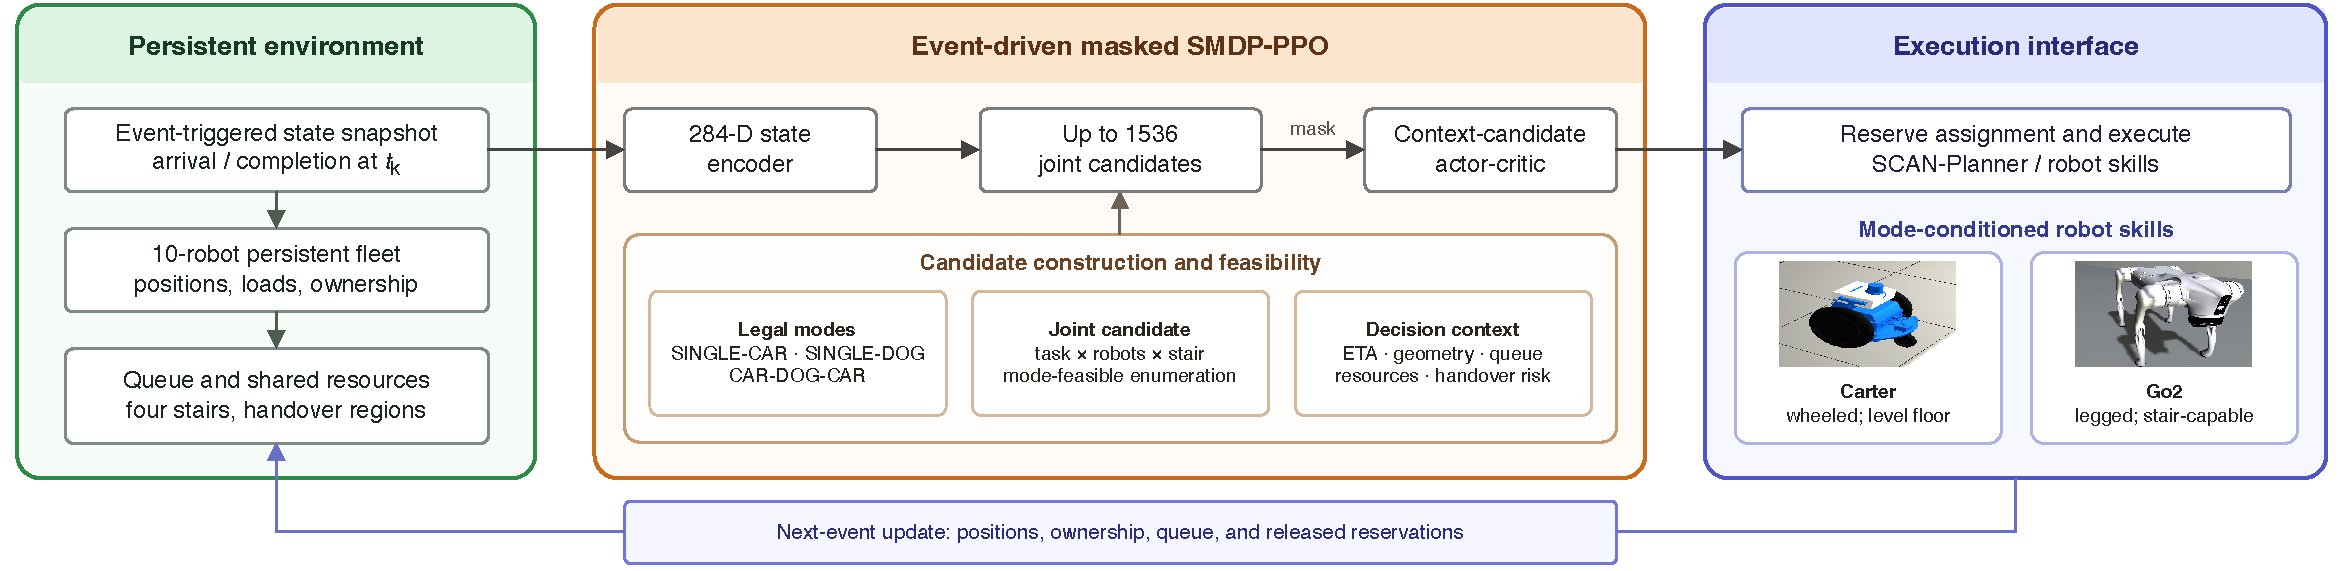
\includegraphics[width=\textwidth]{figures/fig_architecture_drawio.pdf}
\caption{Event-driven masked SMDP-PPO and its simulator interfaces. At each event, the policy scores only legal task--mode--robot--stair candidates; the selected assignment is executed by morphology-specific navigation skills, and the persistent system state returns at the next event. Insets are project-generated model views, not hardware evidence.}
\label{fig:architecture}
\end{figure*}

\subsection{SMDP Definition}

Decision epoch $k$ occurs at simulated time $t_k$. The tuple
$(s_k,a_k,r_k,\Delta t_k,s_{k+1})$ uses holding time
$\Delta t_k=t_{k+1}-t_k$. The action is
\begin{equation}
 a_k=(i,m,r_{\mathrm{src}},r_d,h,r_{\mathrm{dst}}),
\end{equation}
where $i$ is a visible task, $m$ is a transport mode, $r_{\mathrm{src}}$ and $r_{\mathrm{dst}}$ are optional source- and destination-floor Carter robots, $r_d$ is an optional Go2, and $h$ is an optional stairway. Fields that do not apply to the selected mode are empty. Handover locations follow from $h$, and standby placement is deterministic rather than learned. If no assignment is legal, one controlled \textsc{Wait} action advances time to the next event; waiting is not freely selectable while a feasible task is available.

Time-aware discounting is
\begin{equation}
  \gamma_k=\gamma_0^{\Delta t_k/\tau_\gamma},
  \qquad \gamma_0=0.99,\quad \tau_\gamma=\SI{10}{s}.
  \label{eq:discount}
\end{equation}
The objective is $\mathbb{E}_{\pi}[\sum_k(\prod_{j<k}\gamma_j)r_k]$. Equation~\eqref{eq:discount} ensures that two action sequences spanning the same simulated duration receive comparable discounting even if they contain different numbers of scheduler events.

\subsection{State and Candidate Encoding}

The global state has 284 normalized components:
\begin{equation}
  8 + 8\times13 + 10\times14 + 4\times8 = 284.
\end{equation}
The eight global features encode normalized time, waiting and pending task counts, active-task fraction, execution mode, completion and failure fractions, and the dispatch gap. Up to eight visible tasks contribute floor relation, priority, wait, slack, and source/goal geometry. The complete queue is retained internally; the observation exposes the highest-priority eight tasks, ordered by priority, deadline, waiting time, and identifier. Ten robot slots encode morphology, nominal speed, floor, availability, failure and cargo/task flags, position, accumulated distance, completed-task count, and idle time. Four stair slots encode availability and endpoint geometry.

Each decision contains at most 1536 candidate slots. A 30-D candidate vector includes mode indicators; task, robot, and stair identities; cross-floor status; pickup, legged, source-side, stair, and destination-side time estimates; total estimated cost; task priority, wait, slack, and geometry; cost difference and ratio relative to the cheapest legal candidate for the same task; participant count; handover count; and an estimated handover-timeout probability. Padding slots remain masked.

\begin{table*}[!t]
\centering
\caption{Fixed tensor interface. Multiplicity is shown explicitly for the global state; candidate groups sum to 30 features for each of at most 1536 slots.}
\label{tab:encoding_breakdown}
\footnotesize
\setlength{\tabcolsep}{4.0pt}
\begin{tabular}{p{0.36\textwidth}cp{0.36\textwidth}c}
\toprule
Global-state group & Dimension & Per-candidate group & Dimension \\
\midrule
System time, queue, execution, completion/failure, dispatch gap & 8
& Valid-slot flag and transport-mode indicators & $1+3$ \\
Visible tasks: presence, floors, priority, wait, slack, source/goal xyz & $8\times13=104$
& Task, pickup-Carter, Go2, stair, receiving-Carter slots & 5 \\
Robots: presence, morphology, speed, floor, status, xyz, history & $10\times14=140$
& Cross-floor flag and six ETA/cost estimates & $1+6$ \\
Stairs: presence, availability, two endpoint xyz coordinates & $4\times8=32$
& Priority, wait, slack, and source/goal xyz & $3+6$ \\
\cmidrule(lr){1-2}\cmidrule(lr){3-4}
Total & 284
& Relative cost pair, participant/handover counts, timeout prior & $2+3$ \\
\cmidrule(lr){3-4}
& & Total per candidate & 30 \\
\bottomrule
\end{tabular}
\end{table*}

This factorization gives a stable tensor interface without assigning permanent semantics to an index. Candidate slot 17, for example, may represent different tasks and robot tuples at different epochs. All slot-dependent trainable parameters are therefore shared. Candidate travel times use three-dimensional Euclidean distance divided by nominal robot speed. In \modechain, simultaneous approaches are combined by their critical path rather than summed sequentially; nominal transfer durations and a small completed-task load term are then included in the estimated cost. These are scheduler features, not low-level planned path lengths or energy estimates. A single-transfer timeout prior of 0.05 gives a two-transfer relay prior of $1-(1-0.05)^2=0.0975$.

\subsection{Feasibility Mask}

The candidate generator first applies mode compatibility. Same-floor tasks reject \modechain; cross-floor tasks reject \modecar. A \modedog{}~candidate cannot include a Carter, while a \modecar{}~candidate cannot include a Go2 or stairway. A \modechain{}~candidate requires one Carter on each relevant floor, one Go2, one free stairway, and valid sending and receiving regions.

The mask further excludes busy or failed robots, floor mismatches, robots already carrying cargo, conflicting stair and region reservations, occupied handover points, duplicate standby claims, and cargo-ownership violations. Invalid-action masking is particularly useful when a changing combinatorial catalog contains many infeasible choices~\cite{huang2022masking}. Consequently, the categorical policy distribution is supported only on legal candidates:
\begin{align}
  \tilde{\ell}_{k,j}&=\begin{cases}
    \ell_{k,j}, & M_{k,j}=1,\\
    -\infty, & M_{k,j}=0,
  \end{cases} \label{eq:masked_logits}\\
  \pi(a_k=j\mid s_k)&=\operatorname{softmax}(\tilde{\ell}_k)_j.
  \label{eq:masked_policy}
\end{align}
The mask is a safety and consistency mechanism, not a learned penalty. Illegal assignments are never sampled during training or evaluation.

\subsection{Context--Candidate Actor--Critic}

Let $x_k\in\mathbb{R}^{284}$ be the global state and $c_{k,j}\in\mathbb{R}^{30}$ the $j$th candidate. Two multilayer perceptrons produce 96-D embeddings
\begin{equation}
 z_s=f_s(x_k),\qquad z_{c,j}=f_c(c_{k,j}).
\end{equation}
The actor explicitly combines state, candidate, and their elementwise interaction:
\begin{equation}
 \ell_{k,j}=f_\pi([z_s,z_{c,j},z_s\odot z_{c,j}]).
 \label{eq:actor}
\end{equation}
The interaction term makes candidate quality conditional on queue state, robot positions, geometry, and reservations rather than encouraging one global mode preference. The critic uses only the state embedding, $V(s_k)=f_V(z_s)$. All hidden layers use $\tanh$ activations and width 96. The current network has 86,210 trainable parameters.

\subsection{Reward and SMDP-PPO Update}

For transition interval $[t_k,t_{k+1}]$, let $I_k=\int_{t_k}^{t_{k+1}}N(t)\,dt$ be the outstanding-task time integral, $S_k$, $O_k$, $L_k$, and $F_k$ the numbers of successful, on-time, late, and failed task resolutions, $H_k$ the number of completed handovers, and $B_k$ the occupied robot-seconds. The reward is
\begin{align}
 r_k={}&-\frac{I_k}{30}+2S_k+0.5O_k-2L_k-0.05H_k \nonumber\\
 &-2\times10^{-4}B_k-2F_k,
\label{eq:reward}
\end{align}
where $O_k+L_k=S_k$. A separate unrecoverable-fault transition terminates the episode with a penalty of $-10$. No term rewards a particular transport mode. Distance is recorded as an evaluation metric but its reward coefficient is currently zero to avoid duplicating travel-time cost.

Training uses PPO with clipped probability ratio $\epsilon=0.2$~\cite{schulman2017ppo}. The GAE recursion substitutes the variable discount from~\eqref{eq:discount}:
\begin{align}
 \delta_k &= \hat r_k + \gamma_k V(s_{k+1})-V(s_k),\\
 \hat A_k &= \delta_k+\gamma_k\lambda\hat A_{k+1},\qquad \lambda=0.95.
\end{align}
Bootstrap is cut at episode termination. Training rewards are divided by the running standard deviation of variable-discount returns, without mean subtraction, and clipped to $[-10,10]$; evaluation retains the raw environment reward. PPO uses learning rate $3\times10^{-4}$, four epochs, minibatches of 32, value coefficient 0.5, entropy coefficient 0.01, and gradient-norm limit 1.0. Before PPO, each independent seed initializes only the actor from 400 legal rule demonstrations using 30 supervised epochs, batch size 32, and Adam learning rate $10^{-3}$. The critic is not distilled.

\section{Experimental Protocol}
\label{sec:protocol}

Table~\ref{tab:protocol_parameters} summarizes the frozen workloads, replication counts, fault schedules, and inference boundaries used throughout the three studies.

\subsection{Feature-Ablation Protocol}

The feature-ablation campaign compares the complete 284-D state against five one-group removals: persistent position, ETA/cost, short execution history, explicit queue/resource cues, and explicit handover-risk cues. The final analysis uses fresh locked \textsc{Dense} and \textsc{Burst} streams that were not used for checkpoint selection. Each condition retains ten independently trained policies and evaluates them on the same 100 test seeds per profile. Crossed bootstrap intervals resample training and shared test seeds; exact sign-flip tests are adjusted over the 30 primary feature hypotheses with Holm's procedure. Earlier checkpoint-selection observations are treated as diagnostic and are not pooled with this final test.

\subsection{Study I: Nonstationary Load Adaptation}

Each training episode contains 20 asynchronously released tasks balanced across same-floor, cross-region, upward, and downward transport. Three fixed-profile cohorts are trained under \textsc{Medium}, \textsc{Dense}, and \textsc{Burst} arrival loads. The profile name denotes the training load, not a transport mode: every policy can select \modecar, \modedog, or \modechain{}~at every decision whenever the candidate is legal. Each cohort contains ten independent training seeds with distinct network initialization, rule-distillation warm start, PPO stream, and minibatch order. Every seed runs for 2000 PPO updates. Every update logs the actor loss, value loss, entropy, approximate KL divergence, clip fraction, and their composite PPO objective after averaging over four epochs and all minibatches. At 50-update intervals, the current policy is evaluated on the same 100 profile-matched validation episodes (2000 tasks); these diagnostic streams are disjoint from all final locked tests.

The locked mixed-load test concatenates \textsc{Normal}, \textsc{Dense}, \textsc{Burst}, and \textsc{Recovery} in one 80-task episode, with 20 composition-matched tasks per phase. Only inter-arrival intensity changes; robot positions, cargo ownership, outstanding tasks, and resource reservations persist across phase boundaries. The 30 frozen policies are evaluated on 100 fresh shared test seeds (3000 episodes and 240,000 task records). A time-greedy legal-candidate rule and a single-legged-robot-only control use the same 100 task streams, producing another 200 episodes and 16,000 task records. Task-keyed common random numbers are used for handover sampling.

Primary metrics are task success rate, successful throughput, raw episode return, mean and 95th-percentile waiting time, mean flow time, distance per task, and transport-mode distribution. PPO--baseline differences use 10,000 crossed-bootstrap replicates that resample both training seeds and shared test seeds. Mode adaptation uses the same two-dimensional bootstrap. The time-greedy trajectory in the adaptation figure is descriptive because it has no training-seed dimension. Profile-to-profile comparisons are treated as exploratory.

\subsection{Study II: Mixed-Regime Generalization}

Ten preregistered mixed-curriculum policies are trained in episodes whose persistent load phases are randomized, subject to Burst preceding Recovery. All ten policies---including three that did not pass their training gate---are frozen before testing and retained in the analysis. A separate locked test uses 100 new shared seeds ($64{,}000{,}000$--$64{,}000{,}099$) for the ten mixed policies, all 30 fixed-load policies, the time-greedy rule, and the single-dog control. Each policy and baseline is evaluated on 100 80-task episodes. The audit accounts for 320,000 policy task records, finds no illegal action or resource leak, and verifies a common task fingerprint across methods. Comparisons use 10,000 crossed-bootstrap replicates over training and test seeds.

\subsection{Study III: Compute and Logical-Fault Stress Tests}

Two frozen stress tests are added after training is complete. The scheduling-computation benchmark crosses team sizes $\{4,7,10\}$, stair counts $\{1,2,4\}$, and waiting-queue sizes $\{1,2,4,8,16,32\}$, giving 54 scenarios. Candidate generation, legality masking, complete encoding, policy forward evaluation, and the end-to-end decision are each timed 500 times on one ARM64 CPU thread. These timings remain inside the trained tensor shape: at most ten robots, four stairs, eight visible tasks, and 1536 candidate slots.

The logical-fault test freezes ten mixed-curriculum policies and evaluates each on the same 100 locked test seeds under a no-fault control, task-level navigation failures, temporary stair unavailability, and temporary robot unavailability. The resulting 40 PPO jobs contain 4000 episodes; time-greedy and single-dog controls add eight jobs and 800 episodes. With 80 tasks per episode, the campaign contains 384,000 task records. Fault schedules and task streams are shared within each scenario, and the freeze manifest verifies the policy hashes and absence of locked-test outputs before the protocol is sealed. PPO--baseline intervals again use 10,000 crossed-bootstrap replicates over training and test seeds. These injections alter the logical SMDP state and outcomes; they do not emulate ROS, planner, perception, dynamics, or hardware faults.

\begin{table*}[!t]
\centering
\caption{Core experimental parameters. $U[a,b]$ denotes a continuous uniform inter-arrival interval unless otherwise stated. Every 20-task block has the same task composition.}
\label{tab:protocol_parameters}
\footnotesize
\setlength{\tabcolsep}{4.0pt}
\begin{tabular}{>{\raggedright\arraybackslash}p{0.13\textwidth}>{\raggedright\arraybackslash}p{0.57\textwidth}>{\raggedright\arraybackslash}p{0.23\textwidth}}
\toprule
Component & Frozen setting & Replication or boundary \\
\midrule
Arrival profiles & \textsc{Medium} $U[55,75]$ s; \textsc{Dense} $U[15,25]$ s; \textsc{Normal} $U[80,100]$ s; \textsc{Burst} $U[1,3]$ s & Recovery returns to \textsc{Normal} \\
20-task composition & F1 local/cross-region: 3/2; F2 local/cross-region: 3/2; cross-floor up/down: 5/5 & Composition fixed across phases \\
Priority and deadline & Cross-floor priority 3; same-floor priority $U\{1,2\}$; deadline $a_i+180+U\{0,\ldots,60\}$ s & Task-keyed shared streams in locked tests \\
Handover model & 500 provisional samples per direction; P95 strict-greater-than timeout & Logical calibration, not measured hardware timing \\
Feature ablation & \textsc{Dense}/\textsc{Burst}; full state plus five one-group removals & 10 training seeds $\times$ 100 shared test seeds \\
Study I & \textsc{Normal}$\rightarrow$\textsc{Dense}$\rightarrow$\textsc{Burst}$\rightarrow$\textsc{Recovery}; 80 tasks & 30 frozen policies $\times$ 100 shared streams \\
Study II & Randomized persistent four-phase order, with Burst before Recovery; 80 tasks & 10 frozen policies $\times$ 100 new shared streams \\
Study III latency & 3 team sizes $\times$ 3 stair counts $\times$ 6 queue sizes & 54 scenarios, 500 measurements/component \\
Study III faults & Navigation at 18--43\% and 56--81\% arrivals (0.05/leg, +15 s); stair at 25--40\% and 60--75\%; Carter/Go2 at 20--40\%/55--75\% & 10 policies $\times$ 100 shared seeds/scenario; non-preemptive \\
Inference & Paired/crossed bootstrap over training and test seeds & 10,000 replicates; profile comparisons exploratory \\
\bottomrule
\end{tabular}
\end{table*}

\section{Results}
\label{sec:results}

\subsection{Training Optimization and Stability}

Figure~\ref{fig:training_convergence} reports post-warm-start optimization and validation trajectories. The logged composite objective is $L=L_{\mathrm{actor}}+0.5L_{\mathrm{value}}-0.01\mathcal{H}$. For each seed, Panel~(a) summarizes each non-overlapping 50-update block by its median loss before aggregating across seeds. The Medium median decreases from 0.142 in the first block to 0.043 in the terminal block. Dense changes from 0.082 to 0.080 and Burst from 0.0126 to 0.0117, indicating profile-specific low-loss plateaus rather than continued monotonic decrease. Across all three cohorts, median validation success remains between 96.45\% and 98.03\%. Because PPO targets and on-policy rollout distributions change during training, and because the three profiles generate different rollouts, absolute loss magnitude is an optimization diagnostic rather than a cross-profile performance ranking. Every formal locked test therefore uses the preregistered terminal policy and is interpreted using task-level metrics, not retrospective selection of a low-loss checkpoint.

\begin{figure}[!t]
\centering
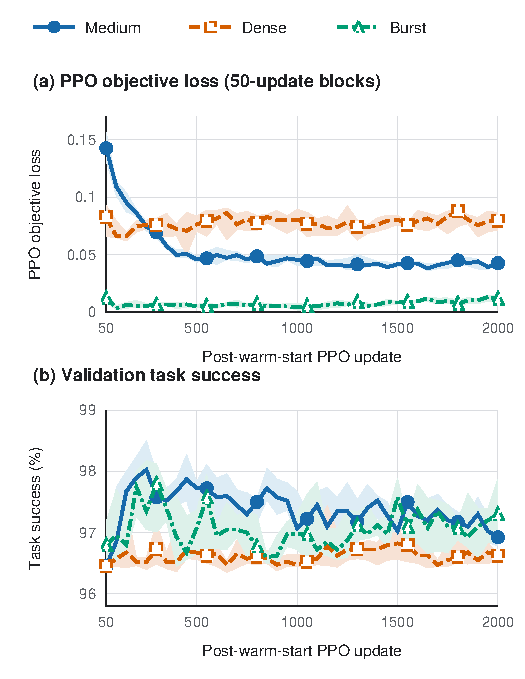
\includegraphics[width=\columnwidth]{figures/fig_training_convergence.pdf}
\caption{Post-warm-start PPO optimization and validation trajectories. Panel (a) plots the composite objective $L=L_{\mathrm{actor}}+0.5L_{\mathrm{value}}-0.01\mathcal{H}$; each point is a per-seed median over one non-overlapping 50-update block. Panel (b) evaluates 100 profile-matched episodes per seed every 50 updates. Lines and bands are medians and interquartile ranges over ten seeds. Loss magnitude is not a cross-profile performance ranking, and validation streams are disjoint from the final locked tests.}
\label{fig:training_convergence}
\end{figure}

\subsection{Feature Contribution on Fresh High-Load Streams}

Table~\ref{tab:feature_ablation} reports the final locked feature-ablation family. Removing ETA/cost cues produces the only large and directionally consistent degradation: the complete state improves return by 24.83 in \textsc{Dense} and 40.84 in \textsc{Burst}, while success rises by 1.97 and 1.60 percentage points, respectively. All ten seed-level differences favor the complete state for these four comparisons, and their crossed-bootstrap intervals exclude zero. The family-wise Holm-adjusted value is nevertheless 0.0586 (global Holm 0.109), just above 0.05, so we describe ETA/cost as the strongest and most consistent contribution rather than claiming confirmatory significance after the full multiplicity correction.

The position, history, explicit queue/resource, and explicit handover-risk removals have small effects with intervals crossing zero in both profiles. An earlier checkpoint-selection run showed a qualitative mode collapse when persistent position was removed, but the final fresh locked tests did not reproduce a stable independent position effect. We therefore retain that observation only as a diagnostic, not as confirmatory evidence.

\begin{table*}[!t]
\centering
\caption{Fresh locked feature ablation. Entries are complete-state minus ablated-policy differences with crossed-bootstrap 95\% CIs over ten training and 100 shared test seeds. Positive return and success differences favor the complete state. Success is in percentage points.}
\label{tab:feature_ablation}
\scriptsize
\setlength{\tabcolsep}{3.1pt}
\begin{tabular}{lrrrr}
\toprule
Removed feature group & \textsc{Dense} $\Delta$ return & \textsc{Dense} $\Delta$ success & \textsc{Burst} $\Delta$ return & \textsc{Burst} $\Delta$ success \\
\midrule
Persistent position & $0.25\;[-0.29,0.83]$ & $-0.09\;[-0.35,0.16]$ & $-0.23\;[-1.17,0.78]$ & $0.13\;[-0.19,0.51]$ \\
ETA/cost context & $\mathbf{24.83\;[22.78,26.92]}$ & $\mathbf{1.97\;[1.35,2.64]}$ & $\mathbf{40.84\;[36.89,44.92]}$ & $\mathbf{1.60\;[1.02,2.23]}$ \\
Execution history & $-0.10\;[-0.58,0.43]$ & $0.02\;[-0.31,0.37]$ & $0.32\;[-0.59,1.23]$ & $0.09\;[-0.30,0.51]$ \\
Queue/resource cues & $0.21\;[-0.35,0.80]$ & $0.02\;[-0.19,0.22]$ & $0.52\;[-0.68,1.72]$ & $0.09\;[-0.16,0.40]$ \\
Handover-risk cues & $0.05\;[-0.40,0.52]$ & $-0.33\;[-0.71,0.04]$ & $0.28\;[-0.72,1.26]$ & $-0.11\;[-0.51,0.27]$ \\
\bottomrule
\end{tabular}
\end{table*}

\subsection{Study I: Nonstationary Load Adaptation}

\subsubsection{Locked-Test Integrity and Absolute Performance}

The formal data audit found no task-stream fingerprint mismatch, duplicate PPO task key, illegal action, or resource leak. All 240,000 PPO tasks were accounted for, and no PPO episode terminated with unresolved tasks. Table~\ref{tab:stage19_absolute} reports absolute locked-test performance. The three PPO rows average over ten training seeds and 100 test seeds; each baseline row averages over the 100 shared test seeds. Raw return is negative because outstanding-task cost accumulates throughout the 80-task episode, so it is meaningful only under this common protocol.

\begin{table*}[!t]
\centering
\caption{Absolute performance in the continuous \textsc{Normal}$\rightarrow$\textsc{Dense}$\rightarrow$\textsc{Burst}$\rightarrow$\textsc{Recovery} locked test. Waiting and flow times are in seconds, throughput is in successful tasks/h, and distance is normalized per task. PPO cohort names denote the load used during training.}
\label{tab:stage19_absolute}
\footnotesize
\setlength{\tabcolsep}{3.4pt}
\begin{tabular}{lrrrrrrr}
\toprule
Method & Success (\%) & Return & Throughput & Mean wait & P95 wait & Mean flow & Distance/task \\
\midrule
PPO--Medium & 99.159 & -431.94 & 71.62 & 166.02 & 659.34 & 210.43 & 50.87 \\
PPO--Dense  & 97.990 & -313.01 & 70.80 & 124.96 & 519.09 & 168.32 & 60.91 \\
PPO--Burst  & 98.066 & -308.35 & 70.85 & 123.03 & 503.34 & 166.30 & 60.07 \\
Time-greedy rule & 97.087 & -457.12 & 70.16 & 173.38 & 727.11 & 216.04 & 71.09 \\
Single-dog only  & 96.938 & -935.09 & 69.82 & 330.87 & 1286.68 & 387.41 & 45.23 \\
\bottomrule
\end{tabular}
\end{table*}

\subsubsection{Paired Comparison With the Time-Greedy Rule}

Figure~\ref{fig:stage19_paired} reports PPO minus time-greedy differences. All three cohorts improve success and successful throughput with 95\% confidence intervals excluding zero. The Medium cohort gains 2.071 percentage points in success (95\% CI [1.749, 2.403]) and 1.458 tasks/h in throughput ([1.236, 1.695]). Dense and Burst gain 0.903 and 0.979 percentage points in success and 0.636 and 0.693 tasks/h in throughput, respectively.

The waiting-time evidence is load dependent. Dense reduces mean waiting by 48.42~s ([-53.72, -43.24]) and P95 waiting by 208.02~s ([-233.75, -182.40]); Burst reduces them by 50.36~s ([-55.61, -45.10]) and 223.77~s ([-249.28, -198.21]). Medium reduces P95 waiting by 67.77~s ([-118.51, -18.61]), but its mean-wait difference of -7.37~s has an interval crossing zero ([-19.76, 4.34]). We therefore do not claim a mean-wait improvement for Medium.

\begin{figure*}[!t]
\centering
\IfFileExists{figures/fig_stage19_paired_differences.pdf}
  {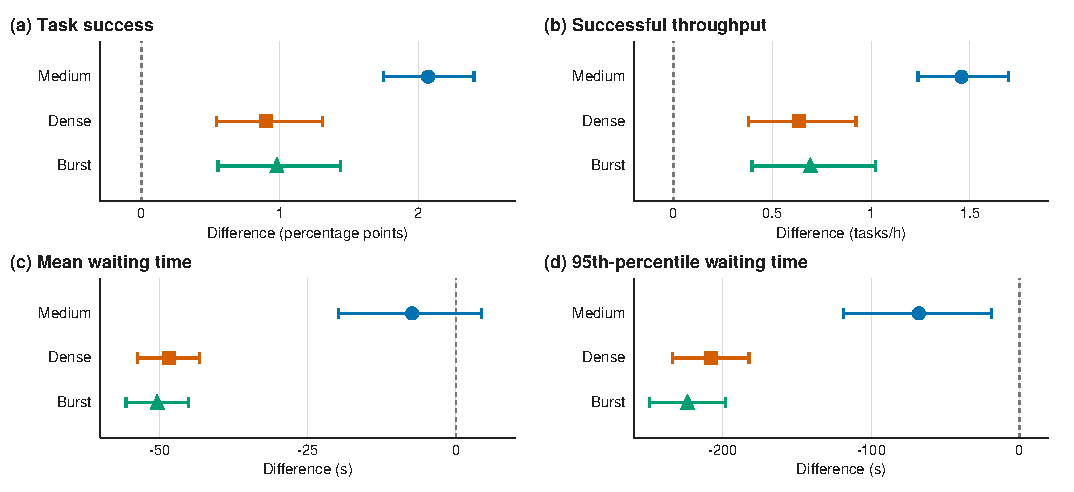
\includegraphics[width=\textwidth]{figures/fig_stage19_paired_differences.pdf}}
  {\StagePairedFallback}
\caption{Paired locked-test differences relative to the time-greedy rule. Markers are point estimates and bars are crossed training-seed--test-seed bootstrap 95\% confidence intervals (10,000 replicates). Positive values favor PPO for success and throughput; negative values favor PPO for waiting time.}
\label{fig:stage19_paired}
\end{figure*}

\subsubsection{Mode Adaptation and Recovery}

Figure~\ref{fig:stage19_adaptation}(a) shows that the learned scheduler does not commit to one transport mode. From Normal to Burst, the share of \modechain{}~decreases from 20.71\% to 5.17\% for Medium, from 32.22\% to 19.88\% for Dense, and from 31.62\% to 18.87\% for Burst. The corresponding Burst-minus-Normal changes are -15.54 percentage points ([-18.01, -12.98]), -12.35 ([-15.18, -9.44]), and -12.75 ([-15.84, -9.81]). Because task composition is held fixed across phases, these changes reflect a response to the persistent queue and resource state rather than a change in task mix. The time-greedy rule changes by only -1.85 percentage points and is shown descriptively.

Recovery is quantified at the task level by the mean waiting time of the last ten Recovery arrivals minus that of the first ten. Figure~\ref{fig:stage19_adaptation}(b) gives -174.90~s for Medium ([-201.89, -147.45]), -93.84~s for Dense ([-101.35, -86.93]), and -104.07~s for Burst ([-114.24, -94.02]). All intervals remain below zero, showing that waiting decreases during the recovery phase. This is evidence of queue clearance under the stated 20-task recovery window, not a control-theoretic settling-time guarantee.

\begin{figure*}[!t]
\centering
\IfFileExists{figures/fig_stage19_adaptation_recovery.pdf}
  {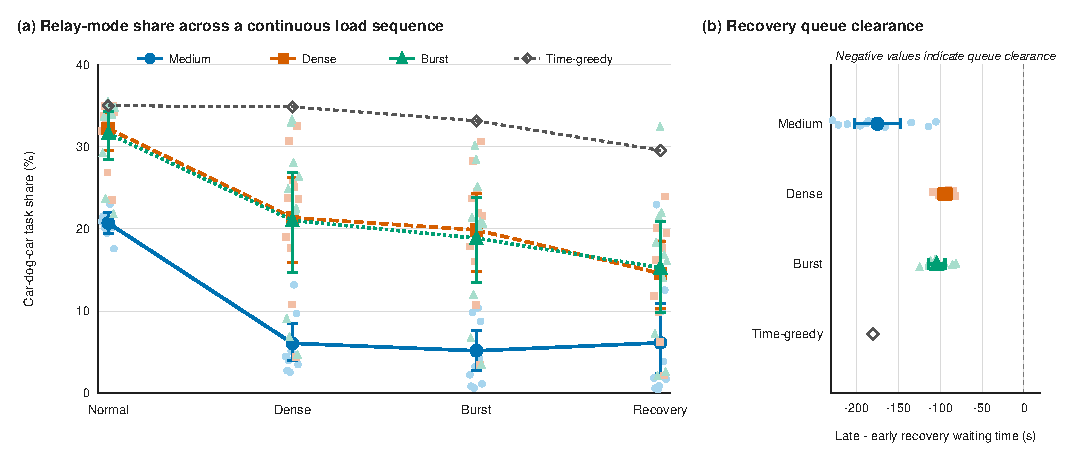
\includegraphics[width=\textwidth]{figures/fig_stage19_adaptation_recovery.pdf}}
  {\StageAdaptFallback}
\caption{Behavior under a continuous four-phase load sequence with no state reset. (a) \modechain{}~share; solid symbols are cohort means and bars are crossed-bootstrap 95\% confidence intervals. The gray time-greedy line is descriptive. (b) Recovery waiting-time change, defined as the last ten minus the first ten Recovery arrivals; negative values indicate queue clearance.}
\label{fig:stage19_adaptation}
\end{figure*}

\subsection{Study II: Mixed-Regime Generalization}

Table~\ref{tab:stage20_absolute} reports absolute mixed-regime performance, and Figure~\ref{fig:stage20_generalization} summarizes the corresponding paired tradeoffs.

\begin{table*}[!t]
\centering
\caption{Absolute performance on the Study II randomized persistent mixed-load test. All policy rows use ten frozen training seeds and 100 shared test streams; rule controls use the same 100 streams. Waiting times are in seconds.}
\label{tab:stage20_absolute}
\footnotesize
\setlength{\tabcolsep}{4.0pt}
\begin{tabular}{lrrrrrr}
\toprule
Method & Success (\%) & Return & Throughput (task/h) & Mean wait & P95 wait & Distance/task \\
\midrule
Mixed-curriculum PPO & 96.514 & -292.41 & 68.401 & 116.60 & 466.18 & 72.12 \\
Medium specialist & 99.008 & -353.42 & 70.001 & 139.54 & 555.18 & 52.65 \\
Dense specialist & 97.774 & -264.76 & 69.257 & 109.61 & 449.17 & 62.34 \\
Burst specialist & 97.708 & -258.68 & 69.207 & 107.21 & 433.14 & 61.97 \\
Time-greedy rule & 96.475 & -381.87 & 68.353 & 146.74 & 599.00 & 72.56 \\
Single-dog only & 96.888 & -840.65 & 68.237 & 295.49 & 1155.17 & 46.40 \\
\bottomrule
\end{tabular}
\end{table*}

\begin{figure*}[!t]
\centering
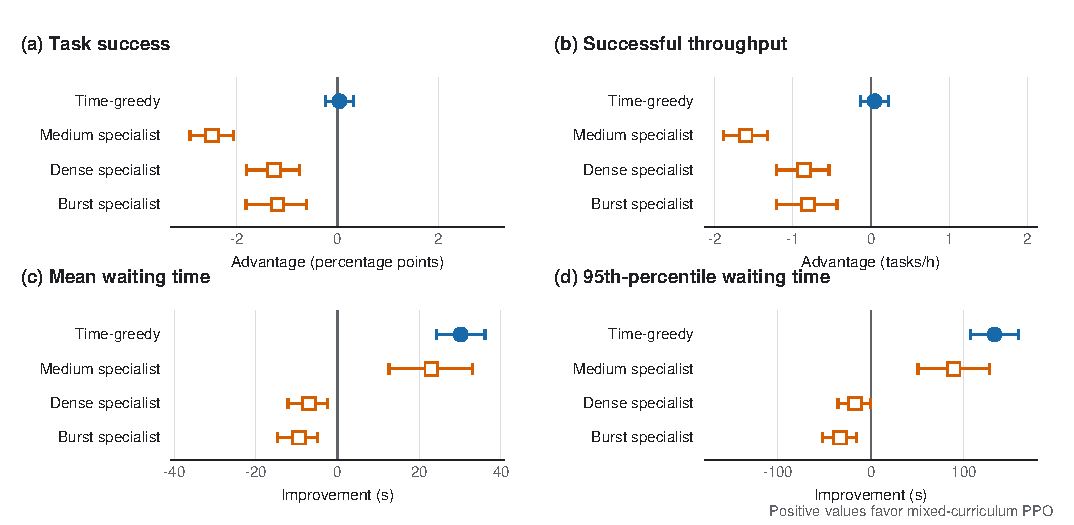
\includegraphics[width=\textwidth]{figures/fig_stage20_generalization.pdf}
\caption{Mixed-curriculum generalization relative to the time-greedy rule and three fixed-load specialists. For success and throughput, points are mixed PPO minus comparator; for waiting time, points are comparator minus mixed PPO. Thus, positive values consistently favor the mixed policy. Whiskers are 95\% intervals from 10,000 crossed-bootstrap replicates over training and shared test seeds. The single-dog control remains in Table~\ref{tab:stage20_absolute} but is omitted here because its much larger waiting differences would compress the specialist comparisons.}
\label{fig:stage20_generalization}
\end{figure*}

The mixed-curriculum cohort achieves 96.514\% success, a mean-episode successful throughput of 68.401 tasks/h, 116.60~s mean waiting, 466.18~s mean episode-level P95 waiting, and 72.12 distance units per task on the randomized persistent mixed-load test. Relative to time-greedy, its success difference is 0.039 percentage points (95\% CI [-0.239, 0.320]) and its throughput difference is 0.048 tasks/h ([-0.135, 0.226]); neither interval excludes zero. It nevertheless improves raw return by 89.46 ([69.98, 108.63]), reduces mean waiting by 30.14~s ([24.28, 36.09]), and reduces episode-level P95 waiting by 132.82~s ([106.77, 158.32]).

Relative to the single-dog control, success and throughput again have intervals crossing zero, whereas return improves by 548.23 ([497.91, 601.45]) and mean waiting falls by 178.88~s ([160.88, 198.10]). This waiting advantage is accompanied by 25.72 additional distance units per task ([23.76, 27.78]). The mixed policy also does not universally dominate load-matched specialists: it improves return and mean waiting relative to the Medium cohort but is worse on success, throughput, and distance, and the Dense and Burst specialists remain more efficient on the evaluated metrics. We therefore interpret this study as evidence that one policy remains competitive across randomized operating regimes, not as evidence that mixed-curriculum training eliminates the value of load specialization.

\subsection{Study III: Compute and Logical-Fault Stress Tests}

Study III evaluates fixed-shape scheduling latency and the response to observable logical failures. Each evidence panel is introduced with its corresponding analysis below.

\subsubsection{Scheduling Latency Within the Trained Shape}

Figure~\ref{fig:stage21_latency} reports the CPU benchmark. With four stairs, end-to-end p99 latency increases with the number of robots and visible waiting tasks, then plateaus once the top-eight visibility cap is reached. Queue sizes 16 and 32 therefore test fixed-shape saturation; they do not establish lossless awareness of tasks outside the visible set. Across all 54 combinations, the largest component p99 values are 0.980~ms for candidate generation, 1.091~ms for legality masking, 3.679~ms for the complete encoder, 1.359~ms for policy forward evaluation, and 4.815~ms end to end. The worst case is the ten-robot, four-stair, 16-waiting-task scenario and remains below the prespecified 100~ms engineering budget. The component timers overlap---the complete encoder includes candidate generation and masking, and the end-to-end timer includes encoding and policy evaluation---so their maxima must not be added.

\begin{figure*}[!t]
\centering
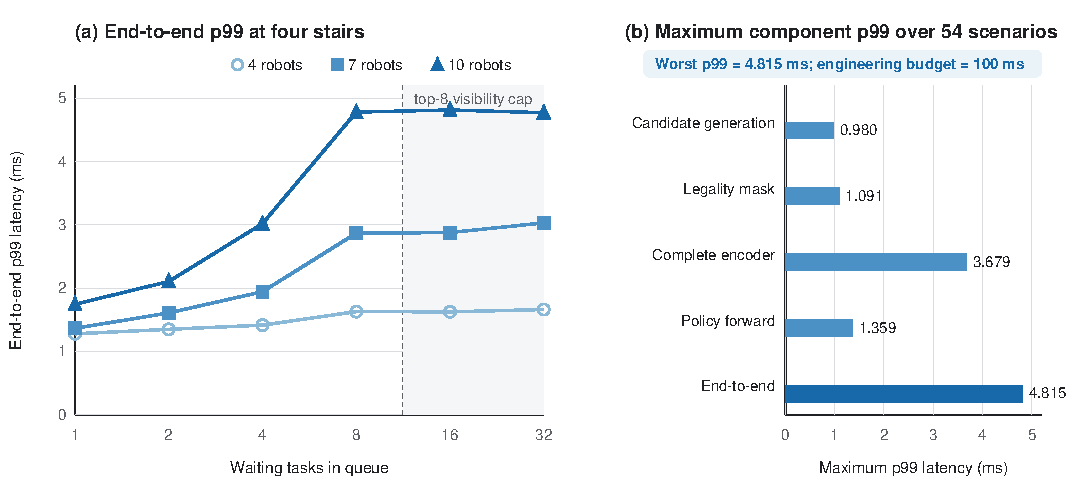
\includegraphics[width=0.89\textwidth,trim=0 5 0 8,clip]{figures/fig_stage21_latency_scaling.pdf}
\caption{CPU scheduling latency within the trained fixed shape. (a) End-to-end p99 with four stairs (500 measurements per point); shading marks queues beyond the eight-task visibility cap. (b) Maximum component p99 across 54 scenarios. Component timers overlap; navigation, ROS communication, and actuation are excluded.}
\label{fig:stage21_latency}
\end{figure*}

\subsubsection{Waiting-Time Effects Under Logical Fault Injection}

Under the no-fault control, mixed-curriculum PPO achieves 96.740\% task success, 68.600 successful tasks/h, 105.28~s mean waiting, and 446.39~s P95 waiting. Time-greedy achieves 96.725\%, 68.579 tasks/h, 137.70~s, and 580.80~s, respectively. The success and throughput differences between PPO and time-greedy have intervals crossing zero, so we treat them as comparable rather than claiming an improvement.

Figure~\ref{fig:stage21_fault} gives the formal waiting-time effects. Relative to time-greedy, PPO reduces mean waiting by 32.42~s in the control, 34.43~s under navigation failures, 32.16~s during stair outages, and 29.76~s during robot outages; all four crossed-bootstrap 95\% intervals exclude zero. The corresponding P95 reductions are 134.41, 138.51, 129.76, and 122.65~s. Improvements relative to the single-dog control are larger, with mean-wait reductions of 190.57--213.95~s and P95 reductions of 695.78--794.77~s.

\begin{figure*}[!t]
\centering
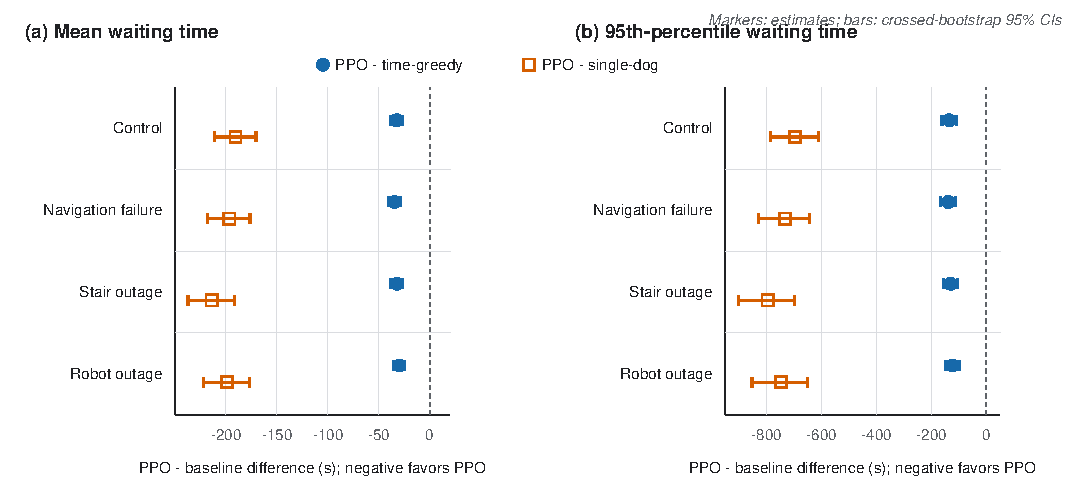
\includegraphics[width=0.89\textwidth,trim=0 5 0 8,clip]{figures/fig_stage21_fault_waiting_effects.pdf}
\caption{Paired waiting-time effects of mixed-curriculum SMDP-PPO versus time-greedy and single-dog controls in four logical scenarios. Markers and whiskers give PPO-minus-baseline estimates and crossed-bootstrap 95\% CIs (ten policies, 100 shared locked seeds, and 10,000 replicates); negative values favor PPO. Faults act at the logical SMDP layer, not in ROS, SCAN-Planner, perception, dynamics, or hardware.}
\label{fig:stage21_fault}
\end{figure*}

Within PPO, temporary stair and robot outages do not produce a significant success or throughput decrease relative to the control, although mean waiting increases by 2.41~s ([1.48, 3.43]) and 3.69~s ([2.50, 4.94]), respectively. Task-level navigation failure is the strongest tested disturbance: PPO success decreases by 8.04 percentage points ([-8.78, -7.35]) and mean waiting increases by 6.36~s ([4.93, 7.95]). This is evidence about the scheduler's response to observable logical failures and resource outages, not physical fault tolerance.
\section{Limitations and Scope}
\label{sec:limitations}

The present implementation evaluates high-level scheduling in a logical continuous-time simulator. Cargo attachment and transfers use transactional ownership rather than contact dynamics. Handover duration is sampled from a reproducible simulation model and is not yet a hardware-measured distribution. Existing community-port SCAN-Planner gates use fixed waypoint routes, a static point cloud, and open-loop kinematic trajectory replay; the learned scheduler has not yet driven randomized closed-loop SCAN missions. Study III navigation failures and resource outages are logical state interventions rather than ROS, planner, perception, dynamics, or hardware faults. The policy therefore should not be interpreted as improving locomotion, manipulation, low-level collision avoidance, or physical fault tolerance.

The fixed-size encoder supports ten robots, four stairs, eight visible tasks, and 1536 candidate slots. Larger teams or denser candidate sets would require either larger tensors or a set/graph representation. Finally, centralized state and deterministic candidate construction assume reliable fleet-state aggregation. Communication delays and partial observability remain future work.

\section{Conclusion}
\label{sec:conclusion}

We presented an event-driven formulation for persistent heterogeneous transport in a multi-floor warehouse. The approach couples task selection, transport-mode choice, robot assignment, and stair reservation in one masked candidate action. A shared context--candidate actor avoids index-specific action parameters, while duration-aware discounting aligns PPO updates with elapsed execution time. In locked logical-simulation tests, fixed-load policies adapted relay use and cleared accumulated waiting under nonstationary load, while a separately trained mixed-curriculum cohort retained competitive success and substantially lower waiting than both rule controls on randomized persistent mixed load. The same ten mixed-curriculum policies subsequently retained waiting-time advantages in a no-fault control and three logical fault conditions, while the worst fixed-shape CPU scheduling p99 remained 4.815~ms. Load-matched specialists nevertheless remained more efficient on some metrics, so the evidence supports coverage across operating regimes rather than universal dominance by one policy. These results establish multi-seed scheduling, computational-latency, and logical-fault evidence, but not navigation, contact-dynamics, or hardware validity. Future work will integrate randomized closed-loop SCAN-Planner execution, measure physical handover distributions, and test communication, perception, and robot failures on hardware.

% Flush the two remaining Study III evidence floats before the bibliography,
% while allowing Limitations and Conclusion to fill the preceding text page.
\FloatBarrier

\bibliographystyle{IEEEtran}
\bibliography{references}

\end{document}
